\documentclass[12pt]{article} % \documentclass{} is the first command in any LaTeX code.  It is used to define what kind of document you are creating such as an article or a book, and begins the document preamble

\usepackage{amsmath} % \usepackage is a command that allows you to add functionality to your LaTeX code

\usepackage[papersize={216mm,330mm},tmargin=20mm,bmargin=20mm,lmargin=20mm,rmargin=20mm]{geometry}
\usepackage[english]{babel}
\usepackage[utf8]{inputenc}
\usepackage{amsmath,amssymb,mathabx,amsthm}%\for eqref
\usepackage{lscape}
\usepackage{graphicx}
\usepackage{tikz}\usetikzlibrary{arrows.meta,calc} %library tikz
\usepackage{subcaption}


\usepackage{pgfplots}
\pgfplotsset{compat=1.15}
\usepackage{mathrsfs}
\usetikzlibrary{arrows}

\usepackage{color,soul} %package for highlining
\usepackage[colorinlistoftodos]{todonotes}
\usepackage{fancyhdr}
\usepackage{hyperref} %creat hyperlink
\hypersetup{
    colorlinks=true,
    linkcolor=blue,
    filecolor=magenta,      
    urlcolor=cyan,
    pdftitle={Overleaf Example},
    pdfpagemode=FullScreen,
    } %set up a hyperlink to be in blue 
\newtheorem{definition}{Definition}[section]
\newtheorem{theorem}[definition]{Theorem}
\newtheorem{prop}[definition]{Proposition}
\newtheorem{lemma}[definition]{Lemma}
\newtheorem{example}[definition]{Example}

\newtheorem*{remark}{Remark}

\pagestyle{fancy}
\cfoot{\thepage} % this is for the page numbering
\setlength\parindent{0pt} % noindent for the whole document.
\renewcommand{\baselinestretch}{1.1} % increase the distance between line.

\DeclareMathOperator{\SLn}{\text{SL}_n(\mathbb{R})}
\DeclareMathOperator{\slnz}{SL_n(\mathbb{Z})}
\DeclareMathOperator{\glnz}{GL_n(\mathbb{Z})}
\DeclareMathOperator{\vol}{vol}

\DeclareMathOperator{\SO}{SO_n(\mathbb{R})}
\newcommand{\tpoint}[1]{\subsection{#1}}

\newcommand{\spoint}{\subsection{}}



\title{CHAPTER  :SEMI-STABLE LATTICE IN HIGHER RANK} % Sets article title
\date{\today} % Sets date for date compiled
\begin{document}
\maketitle % creates a title using the information in the preamble (title, author, date)
In this chapter, we will establish the notion of semi-stable lattice. Heuristically,
this is the lattice that achieve all the successive minima at the same time, see \cite{}.

We will provide two different definitions of semi -stable lattice: one is geometric - which follows Grayson's idea of utilizing
the canonical plot, and one is purely algebraic, which make use of the maximal standard parabolic subgroups.
The toy model will be the moduli space of 2-dimensional lattice, which is essential the upper half plane in the complex field.
At the end, we will show that the two definitions coincide.
\section{Lattices in higher rank}
For each $z$ with $\Im(z)>0$, we can attach to $z$ a lattice structure $L_z = \mathbb{Z}z \oplus \mathbb{Z}$. Roughly speaking
a lattice is a discrete  subgroup that is generated by a $k-$ basis of the $k$-space $V$.
In particular, we will only work with the real vector space $V$. Grayson works with lattice over a ring of algebraic integers, but we will restrict to
just the lattice that has the underlying structure as a $\mathbb{Z}-$ module.

\tpoint{First definition of lattices}
\begin{definition}[\label = Abstract $\mathbb{Z}$-lattices]
    Let $L$ be a finitely generated $\mathbb{Z}$-module. In particular, it is a free $\mathbb{Z}$-module
    of finite rank. Suppose that $L$ is endowed with a real-valued  positive definite\footnote{The non-degenerate implicity state that rank L is the same as $dim L_\mathbb{R}$} quadratic form $Q\colon L \to \mathbb{R}$, such that the set
    \[\left\lbrace x \in L: Q(x) \le r\right\rbrace \]
    is finite for any real number $r$.
    We will call  the pair $(L,Q)$ a \textbf{abstract $\mathbb{Z}$-lattice}.
\end{definition}

An easy example is to take $L = \mathbb{Z}^n$ and choose our quadratic form to be the standard one. namely
\[\left\langle x,y \right\rangle = x \cdot y = \sum_{i=1}^n x_iy_i\]
Here the multiplication is just the usual dot product between 2 vectors. In term of matrix, this quadratic form is assigned to the
identity matrix $I_n$.

If there is no further confusion, we can just denote a Euclidean lattice by $L$, without specifying the bilinear form
$Q$. The lattice $L$ determines a full-rank lattice inside $L_\mathbb{R}$, namely, the rank
of the lattice $L$ is equal to the dimension of $L_\mathbb{R}$.

\tpoint{An alternative definition of lattices}
For the sake of computation, we also usually adopt another definition of the lattice.
In particular, we view lattice as a free $\mathbb{Z}-$ module of rank $n$ that is isomorphic
to $\mathbb{R}^n$ via base changing.
\begin{definition}\label{lattice2}
    A \textit{lattice} in $\mathbb{R}^n$ is a subset $L \subset \mathbb{R}^n$ such that there exists
    a basis $b_1,\ldots,b_n$ of $\mathbb{R}^n$ such that
    \[L = \mathbb{Z}b_1\oplus \mathbb{Z}b_2\oplus \ldots \mathbb{Z}b_n\]
    If we put the vector $b_1,b_2,\ldots,b_n$ in columns, with respect to the standard basis, namely
    \[g = [b_1 | b_2 | \ldots | b_n] ,\]
    then $L = g\mathbb{Z}^n$.
\end{definition}
In the second definition, we can just identify $L$ with the standard lattice $\mathbb{Z}^n$ and the
symmetric positive definite form is $g^tg$. So an Euclidean $\mathbb{Z}$-lattice is an abstract lattice with the standard
positive definite quadratic form.
\tpoint{Equivalence between two definitions of lattices}
In this subsection, we will show that every abstract $\mathbb{Z}$- lattice is isomorphic to an Euclidean $\mathbb{Z}-$ lattice.
This will be helpful in visualizing the abstract lattices, as we are just looking at concrete lattices with deformation by a linear transformation.

First we need to specify the notion of isomorphic lattices - in the first definition
\begin{definition}
    A map $f \colon (L,Q)   \to (L',Q')$  is an \textbf{isomorhism} between lattices if it is a group isomorphism and
    for all $x \in L$, we have
    \[Q(x) = Q'(f(x)) \]
\end{definition}
\begin{prop}\label{equiv-def}
    Any abstract lattice is isomorphic to a Euclidean $\mathbb{Z}-$ lattice.
\end{prop}
\begin{proof}
    Let $(L,Q)$ be an arbitrary lattice. We define a bilinear form as
    \[ \left\langle x,y \right\rangle := \dfrac{Q(x+y)-Q(x-y)}{4}\]
    We will show that this bilinear form defines an inner product over the real vector space $L_\mathbb{R} = L \otimes_\mathbb{Z} \mathbb{R}$.
    Clearly we have $\left\langle x,x \right\rangle = 4Q(x)/4 = Q(x) \ge 0$ for all $x  \in L \setminus \left\lbrace 0 \right\rbrace$.
    Now the extended bilinear form is defined as
    \begin{align*}
        \left\langle \cdot,\cdot \right\rangle  \colon L_\mathbb{R} \times L_\mathbb{R} & \to      \mathbb{R}                      \\
        (x\otimes a, y \otimes b)                                                       & \mapsto  ab\left\langle x,y\right\rangle
    \end{align*}
    It is immediate that the extended bilinear form is inner product. So we have proved that
    $L_\mathbb{R}$ is a Euclidean space containing $L$. Moreover, $L$ is embedded injectively in $L_\mathbb{R}$
    as $\mathbb{R}$ is a flat $\mathbb{Z}$ module. The condition that
    \[ \# \left\lbrace x \in L: Q(x) \le r\right\rbrace < \infty\]
    implies $L$ can be identified with a discrete in $L_\mathbb{R}$. But this implies that there exists a basis
    $\left\lbrace b_1,\ldots,b_n\right\rbrace \subset L_\mathbb{R}$  such that
    \[L = \mathbb{Z}b_1\oplus \mathbb{Z}b_2\oplus \ldots \mathbb{Z}b_n\]
    Hence we are done.\todo{fix the proof so that we use the definition 1.4.}
\end{proof}
\tpoint{Covolume of a lattice}
Now that for every abstract lattice $L$ we can find an invertible matrix $g$ such that
\[ L  \cong g\mathbb{Z}^n\]

The number $n$ is called the \textbf{rank} of the lattice $L$.

Let $\left\lbrace e_1,e_2,\ldots,e_n \right\rbrace$ be an orthonormal basis of $L_\mathbb{R} \cong \mathbb{R}^n$ and
\[g = [b_1 | b_2 | \ldots | b_n] .\] The covolume of the lattice
$L$ is defined as
\begin{definition}
    The covolume of $L$ is given by the formulae
    \[\vol(L) = \left|\det(b_i\cdot e_j)\right|\]
\end{definition}
The rank and covolume are invariant numerical values of $L$, as they don't depend on the choice of basis. Indeed, two bases of a rank $n$ lattice $L$
are related by a transformation $g \in \text{GL}_n(\mathbb{Z})$. Clearly this preserves the volume and the rank as a $\mathbb{Z}-$module.


\tpoint{Sublattices}
To work with semi-stable lattice $L$, we need to consider all the sublattices contained inside $L$.
\begin{definition}[\label=sublattice]
    Let $(L,Q)$ be a Euclidean $\mathbb{Z}$-lattice. We say that a $\mathbb{Z}-$submodule $M$ of
    $L$ a \textbf{sublattice} if and only if $L/M$ is torsion free.
\end{definition}
From this definition, we can prove that $M$ is a sublattice of $L$ if it satisfies one of the
following equivalent properties:
\begin{enumerate}
    \item $M$ is a summand of $L$.
    \item every basis of $M$ can be extended to a basis of $L$.
    \item The group $M$ is an intersection of $L$ with a rational subspace of $L_\mathbb{R}$.
\end{enumerate}
We refer to the \cite{} for a proof of these equivalences.
\begin{example}
    If $L = \mathbb{Z}^2$, then any sublattice of $L$ is a primitive vector $u = (a,b)$, i.e
    $\gcd(a,b)=1$. Indeed, $u=(a,b)$ is a sublattice of $\mathbb{Z}^2$ if and only if there exists a vector $v \in \mathbb{Z}^2$
    such that $L = \mathbb{Z}u \oplus \mathbb{Z}v$. With respect to the usual inner product on $\mathbb{R}^2$,
    we have
    \[1 = \vol(\mathbb{Z}^2) = \det \begin{bmatrix}
            a & b \\
            c & d
        \end{bmatrix} = ad-bc\]
    This happens if and only if $\gcd(a,b)=1$.
\end{example}
\section{Semi-stable lattices in Grayson's sense}
\subsection{Grayson's definition}
In this section, we introduce the idea of Grayson in defining \textit{semi-stable} lattices.
In particular, he associates every lattices a plot and its convex hull - called \textit{ profiles}.
An easy observation is that, if $M \subset L$ is a sublattice, then the space $M_\mathbb{R} = M \otimes \mathbb{R}$
is a subspace of $L_\mathbb{R}$, equipped with the restriction of the positive definite symmetric form $Q$ of $L$, hence $M$
is also a lattice of rank not exceeding rank of $L$.
\begin{definition}[\label = slope]
    The slope of a non-zero lattice $L$ is the number
    \[\mu(L) = \dfrac{\log\vol(L)}{\dim L}\]
\end{definition}
\begin{definition}
    Suppose we have a lattice $L$. For any sublattice $M \subset L$, we assign $M$ to a point
    \[l(M) = \left(\dim M, \log\vol(M)\right)\]
    in the plane $\mathbb{R}^2$. The collection of all points $l(M)$ where $M$ ranges over
    all sublattices of $L$ is called \textbf{ the canonical plot} of the lattice $L$. By convention, we assign
    the lattice of zero rank to the origin of the plane.
\end{definition}

\begin{example}
    Add example about computing the volume of sublattices.
\end{example}
The following lemma asserts that, for each vertical axis $x =i$, there is a lowest point.
\begin{lemma}
    Given a lattice $L$ and a number $c$, there exists only a finite number of sublattices $M \subset L$ such that
    $\vol(M)<c$.
\end{lemma}
\begin{proof}
    We will prove by induction on the rank of the sublattices.
    \begin{itemize}
        \item For $r =1$, the collection of all rank $1$ sublattices of $L$ is just the set of all vectors in $L$. So we reduce
              to show that for any $c>0$, the set $B(0,c) \cap L$  has finitely many elements. But this follows immediately from the fact that
              $L$ is a discrete subset of $L_\mathbb{R}$.
        \item Assume that the lemma holds for $r >1$. Assume that
              \[M = \mathbb{Z}m_1\oplus \ldots \mathbb{Z}m_r\]
              is a sublattice of the lattices $L$ of rank $n$. Consider the wedge product $\bigwedge^r L$, then clearly
              $m_1\wedge m_2\ldots \wedge m_r$ is a vector in the lattice  $\bigwedge^r L$.
              By the previous case, there are finitely
              many vectors with bounded length inside lattice. So we only need to show that the map
              \[ M \mapsto \bigwedge^r M \]
              is finite to one, then we are done. But this is clear.
    \end{itemize}
    So the canonical plot is bounded below.
\end{proof}
\begin{definition}
    The boundary polygon of the convex hull of the canonical plot is called \textbf{profile} of the lattice $L$.
\end{definition}
In theory, we can compute the profile by searching for the shortest vector in each of its exterior product, but this computation
is infeasible when the dimension of the lattice grows. Since there are lattices with
arbitrarily large volume of any rank smaller than that of $L$, we add to the side the point $(0,\infty)$ and $(n,\infty)$. The sides
of the profile are therefore two vertical lines. The bottom is just the convex polygonal connecting the origin with the point
$l(L) = (n,\log\vol(L))$, where $n$ is the rank of $L$.
\begin{definition}\label{ss1}
    If the bottom of the profile contains only two points $(0,0)$ and $(n,\log\vol L)$, then the
    lattice $L$ is said to be \textbf{semi-stable}. Otherwise $L$ is said to be \textbf{unstable}.
\end{definition}
Here are the picture of two lattices. The one on the left is semi-stable while the one on the right is unstable.

\begin{figure}[h]
    \centering
    \begin{minipage}{.2\textwidth}
        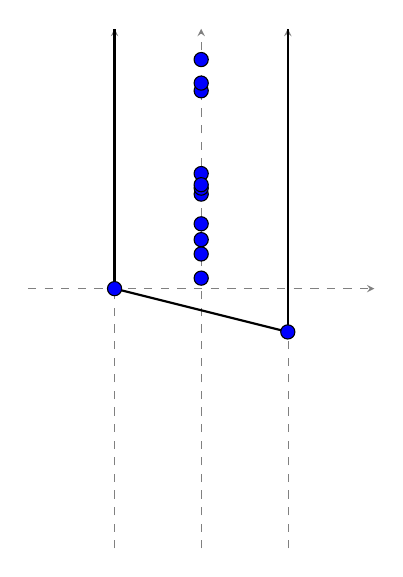
\begin{tikzpicture}[>=stealth, x=1.1cm, y=1.1cm]
            % Dashed lines (axes)
            \draw[help lines, dashed, ->] (-1,0) -- (3,0);
            \draw[help lines, dashed, ->] (0,-3) -- (0,3);
            \draw[help lines, dashed, ->] (1,-3) -- (1,3);
            \draw[help lines, dashed, ->] (2,-3) -- (2,3);
            \draw[thick] (0,0) -- (0,3);
            \draw[thick] (0,0) -- (2, -0.5);
            \draw[thick]  (2,-0.5) -- (2,3);
            \draw[thick]  (2,-0.5) -- (2,3);

            % Points (all with fill=blue and radius=0.09cm)
            \filldraw[fill=blue] (2, -0.5) circle[radius=0.09cm];
            \filldraw[fill=blue] (0, 0) circle[radius=0.09cm]; % Removed duplicate
            \filldraw[fill=blue] (1, 0.12122108098130914) circle[radius=0.09cm];
            \filldraw[fill=blue] (1, 2.28412917072110916) circle[radius=0.09cm];
            \filldraw[fill=blue] (1, 2.3729881287610001) circle[radius=0.09cm];
            \filldraw[fill=blue] (1, 0.4) circle[radius=0.09cm];
            \filldraw[fill=blue] (1, 0.5655158711807637) circle[radius=0.09cm];
            \filldraw[fill=blue] (1, 2.6445016116606668) circle[radius=0.09cm];
            \filldraw[fill=blue] (1, 0.7481703960405396) circle[radius=0.09cm];
            \filldraw[fill=blue] (1, 1.3282219276898275) circle[radius=0.09cm];
            \filldraw[fill=blue] (1, 1.0912647062501184) circle[radius=0.09cm];
            \filldraw[fill=blue] (1, 1.1603772291700336) circle[radius=0.09cm];
            \filldraw[fill=blue] (1, 1.2) circle[radius=0.09cm];
        \end{tikzpicture}~
    \end{minipage} \hspace{3cm} \begin{minipage}{.2\textwidth}
        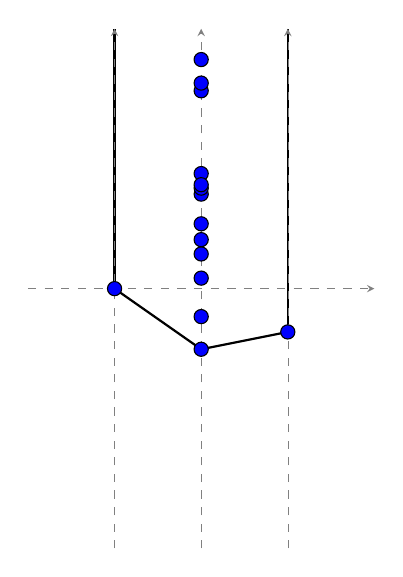
\begin{tikzpicture}[>=stealth, x=1.1cm, y=1.1cm]
            % Dashed lines (axes)
            \draw[help lines, dashed, ->] (-1,0) -- (3,0);
            \draw[thick] (0,0) -- (0,3);
            \draw[thick] (0,0) -- (1, -0.7);
            \draw[thick] (1,-0.7) -- (2,-0.5);
            \draw[thick]  (2,-0.5) -- (2,3);
            \draw[help lines, dashed, ->] (0,-3) -- (0,3);
            \draw[help lines, dashed, ->] (1,-3) -- (1,3);
            \draw[help lines, dashed, ->] (2,-3) -- (2,3);

            % Points (all with fill=blue and radius=0.09cm)
            \filldraw[fill=blue] (2, -0.5) circle[radius=0.09cm];
            \filldraw[fill=blue] (0, 0) circle[radius=0.09cm]; % Removed duplicate
            \filldraw[fill=blue] (1, -0.7) circle[radius=0.09cm];
            \filldraw[fill=blue] (1, -0.3230737092181455) circle[radius=0.09cm];
            \filldraw[fill=blue] (1, 0.12122108098130914) circle[radius=0.09cm];
            \filldraw[fill=blue] (1, 2.28412917072110916) circle[radius=0.09cm];
            \filldraw[fill=blue] (1, 2.3729881287610001) circle[radius=0.09cm];
            \filldraw[fill=blue] (1, 0.4) circle[radius=0.09cm];
            \filldraw[fill=blue] (1, 0.5655158711807637) circle[radius=0.09cm];
            \filldraw[fill=blue] (1, 2.6445016116606668) circle[radius=0.09cm];
            \filldraw[fill=blue] (1, 0.7481703960405396) circle[radius=0.09cm];
            \filldraw[fill=blue] (1, 1.3282219276898275) circle[radius=0.09cm];
            \filldraw[fill=blue] (1, 1.0912647062501184) circle[radius=0.09cm];
            \filldraw[fill=blue] (1, 1.1603772291700336) circle[radius=0.09cm];
            \filldraw[fill=blue] (1, 1.2) circle[radius=0.09cm];
        \end{tikzpicture}~
    \end{minipage}
\end{figure}
Visually, a lattice is called \textbf{semi-stable} if it satisfies the other equivalent
conditions:   If $M$ is an arbitrary sublattice of $L$ then $\mu(M) \ge \mu(L)$.
\subsection{Canonical filtration}
Given a lattice $L$ and a sublattice $M \subset L$, the quotient group $L/M$ have the structure of
a lattice. Indeed, consider the exact sequence of lattices
\[0\rightarrow M\rightarrow L\rightarrow L/M\rightarrow 0\]
By tensoring with $\mathbb{R}$ we get a short exact sequence of $\mathbb{R}$-vector subspaces
\[0\rightarrow M_\mathbb{R} \rightarrow L_\mathbb{R} \rightarrow (L/M)_\mathbb{R}\rightarrow 0,\]
which is split. Thus we have the isomorphisms
\[(L/M)_\mathbb{R} \cong L_\mathbb{R}/M_\mathbb{R} \cong M^\perp_\mathbb{R}\]
Therefore, by restriction of the inner product over $L_\mathbb{R}$ to $M^\perp_\mathbb{R}$, we clearly see that
$L/M$ also inherits an inner product. In particular, it is a lattice.
\begin{definition}
    Given a lattice $L$ containing a sublattice $M$, then $L/M$ is a lattice. We call this lattice \textbf{quotient lattice}.
\end{definition}
\begin{lemma}\label{volume-of-lattice}
    If $L$ is a lattice and $M\subset L$ is a sublattice, we have
    \[\vol(L) = \vol(M)\cdot \vol(L/M)\]
\end{lemma}
\begin{proof}
    Assume that $\{m_i\}$ is a basis for the lattice $M$ and $\{e_i\}$ be an orthonormal basis for the vector space
    $M_\mathbb{R}$. Since $M$ is a sublattice of $L$, we can extend the basis $\{m_i\}$ to get a
    basis $\{m_i\} \cup \{n_j\}$ for the lattice $L$. Similarly, we can extend  $\{e_i\}$ to get an orthonormal
    basis $\{e_i\} \cup \{f_j\}$ for the vector space $L_\mathbb{R}$. In particular, we would have
    $\left\langle m_i,f_j \right\rangle =0$ for all $i,j$.
    By definition, we have
    \begin{align*}
        vol(L) & = \det\begin{bmatrix}
                           \left\langle m_i,e_i\right\rangle  & \left\langle n_j,e_i\right\rangle \\
                           \left\langle m_i,f_J \right\rangle & \left\langle n_j,f_j\right\rangle
                       \end{bmatrix} \\
               & = \det\begin{bmatrix}
                           \left\langle m_i,e_i\right\rangle & \left\langle n_j,e_i\right\rangle \\
                           0                                 & \left\langle n_j,f_j\right\rangle
                       \end{bmatrix}  \\
               & =\vol(M)\cdot \vol(L/M)
    \end{align*}
    Hence we are done.
\end{proof}
In the canonical plot, this 


\section{$\rho$- definition of semi-stability}
We are now ready to define the $\rho$-definition of semi-stable lattice. Recall that
we define the space of lattices of rank $n$ by $X_n := K \backslash \text{GL}_n(\mathbb{R})$, where $K$ is the orthogonal subgroup.
\begin{definition}[\label  = $\rho$-definition]\label{ss2}
    Let $x \in X_n$ be an arbitrary lattice, then the lattice $x$ is called \textbf{semi-stable} if and only if its degree of instability $\deg_{\text{inst}}(x)\ge 0$, where
    \[\deg_{\text{inst}}(x):= \min_{Q \in MaxParSt, \gamma \in \text{GL}(\mathbb{Q})/Q_i(\mathbb{Q})}\left\langle \rho_Q, H_Q(x\gamma) \right\rangle\]
\end{definition}
A simple observation is that - a lattice $x$ is semi - stable if for all maximal standard parabolic subgroups
$Q_i$, we have
\[\min_{\gamma \in \text{GL}_n(\mathbb{Q})/Q_i(\mathbb{Q})}\left\langle \rho_Q, H_Q(x\gamma) \right\rangle \ge 0\]
Note that, in the definition of degree of instability, we can further replace $H_Q$ with $H_B$. This implies that, if
\[ x = kan, \quad k \in K, a \in A, n \in N,\]
as in Iwasawa decomposition, then $H_B(x) = H$ where $H = \exp(a)$. In particular, if
\[a = \begin{bmatrix}
        a_1    & 0      & \ldots & 0      \\
        0      & a_2    & \ldots & 0      \\
        \vdots & \vdots & \vdots & \vdots \\
        0      & 0      & \ldots & a_n
    \end{bmatrix}\]
then
\[\left\langle \rho_{Q_i}, H_B(x) \right\rangle = \dfrac{n}{2}\log(a_1a_2\ldots a_i)\]\todo{Compute this}
Thus, to check for the semi-stability of a lattice $x$, we just need to look at the
$A$-coordinate of $x$, and verify whether the system
\begin{align*}
    \begin{cases}
        a_1 \ge 1   \\
        a_1a_2\ge 1 \\
        \ldots      \\
        a_1a_2\ldots a_n \ge 1
    \end{cases}
\end{align*}
\tpoint{The equivalent between definitions of semi-stable lattices}
So far we have two distinct definitions of semi-stability. The following theorem asserts that they are equivalent:
\begin{prop}
    Let $x \in X_n = K \backslash \text{SL}_n(\mathbb{R})$ - the space of unit lattice. Then $x$ is semi-stable if one of the following equaivalent
    conditions holds
    \begin{enumerate}
        \item The bottom of the profile of $x$ is a line connect solely two points: the origin and $(n,0)$.
        \item The degree of instability of $x$ is nonnegative, namely, $\deg_{inst}(x) \ge 0$.
    \end{enumerate}
\end{prop}
\begin{proof}
    \hfill \\
    If we can prove there is a correspondence between
    $\gamma \in \text{GL}_n(\mathbb{Q})/Q_i(\mathbb{Q})$ and a sublattice of rank $i$ of $x$, then we are done.
    We first need a slight reduction - we identified the quotient $\text{GL}_n(\mathbb{Q})/Q_i(\mathbb{Q})$ with
    the quotient $\text{GL}_n(\mathbb{Z})/(Q_i(\mathbb{Q}) \cap \text{GL}_n(\mathbb{Z})) $. Now let $x$ be an arbitrary lattice of rank $n$.

    We will first show the following correspondence
    \[ \text{GL}_n(\mathbb{Z})/(Q_i(\mathbb{Q}) \cap \text{GL}_n(\mathbb{Z})) \longleftrightarrow \left\lbrace \text{ sublattice of rank $i$ of $\mathbb{Z}^n$}\right\rbrace\]
    We define the map from the collection of sublattices of rank $i$ to the cosets space as follows: For any sublattice $M \subset \mathbb{Z}^n$, there exists
    a basis of $M$, denoted by
    \[\left\lbrace v_1,v_2,\ldots, v_i \right\rbrace \]
    we can extend this basis to get a basis of $\mathbb{Z}^n$
    \[\mathfrak{B'} = \left\lbrace v_1,v_2,\ldots, v_n \right\rbrace \]
    Clearly in $\mathbb{Z}^n$ we have the standard basis $\mathfrak{B} = \left\lbrace e_1,e_2,\ldots,e_n\right\rbrace $. Clearly there
    exists a map $\gamma \in \glnz$ such that
    \[\gamma \cdot e_k = v_k \quad \forall k = 1,2,\ldots, n\]
    So we define the map
    \begin{align*}
        \varphi \colon \left\lbrace\text{sublattices of rank $i$ of $\mathbb{Z}^n$}\right\rbrace & \to \text{GL}_n(\mathbb{Z})/(Q_i(\mathbb{Q}) \cap \text{GL}_n(\mathbb{Z})) \\
        M                                                                                        & \mapsto [\gamma]
    \end{align*}
    where $[\gamma]$ denoted the equaivalent class of $\gamma$ in the quotient space. This is a well-defined map. Indeed, Assume that we extend
    the basis $\mathfrak{B'}$ in a different way to get the basis
    \[ \mathfrak{B}_1 = \left\lbrace v_1,\ldots, v_k, v'_{k+1},\ldots,v'_n \right\rbrace\]
    As above, there also exists $\gamma' \in \glnz$ such that
    \[\gamma' e_k = v_k \quad \forall k \le i, \quad \text{ and } \quad \gamma'e_k = v'_k \quad \forall k > i\]
    But this implies that
    \[(\gamma^{-1})\gamma ' \cdot e_k = \gamma^{-1} v_k = e_k \quad \forall k \le i\]
    So in particular, we have $[\gamma] = [\gamma']$. The inverse map is given by
    \[[\gamma] \mapsto \bigoplus_{k=1}^i\mathbb{Z} (\gamma \cdot e_i) = M\]
    This generalizes in the obvious way for lattice $x = g\mathbb{Z}^n$ for some $g \in \text{GL}_n(\mathbb{R})$. Indeed, we just define
    the map
    \begin{align*}
        \phi_g \colon \left\lbrace\text{sublattices of rank $i$ of $g\mathbb{Z}^n$}\right\rbrace & \to \text{GL}_n(\mathbb{Z})/(Q_i(\mathbb{Q}) \cap \text{GL}_n(\mathbb{Z})) \\
        M_g = gM = g \bigoplus_{k=1}^i  \mathbb{Z}v_i                                            & \mapsto [\gamma]
    \end{align*}
    where $\gamma e_k = v_k$ in $\mathbb{Z}^n$ for all $ k \le i$ and $\phi_g^{-1}([\gamma]) = g \bigoplus_{k=1}^i  \mathbb{Z}(\gamma \cdot e_i)$.
\end{proof}
\todo{Check the map in the generalization carefully - You must show tickmarkheight=
    for the corresponding $\gamma$, it actually compute the volume of the sublattice}
\end{document}






\subsection{$\rho$-definition of semi-stability}
There is another, more algebraic way to determine whether a given lattice is semi-stable.
This definition ultilize the notion of parabolic subgroups.







%Using definition \ref{lattice2}, we have $x = g\mathbb{Z}^n$ for some $g \in \text{GL}_n(\mathbb{R})$.
%Clearly for any sublattice of $x$, called $y$ corresponds to a sublattice of $\mathbb{Z}^n$ via

The precise definition
of a lattice is as follows:
\begin{definition}[\label = Euclidean $\mathbb{Z}$-lattices]
    Let $L$ be a finitely generated $\mathbb{Z}$-module. In particular, it is a free $\mathbb{Z}$-module
    of finite rank. Suppose that $P$ is endowed with a real-valued symmetric positive definite\footnote{The non-degenerate implicity state that rank L is the same as $dim L_\mathbb{R}$} bilinear form, called $Q$.
    Then the space $L_\mathbb{R}= L \otimes_\mathbb{Z} \mathbb{R}$ equipped with the bilinear form $Q$ forms a real
    inner product space. We will call  the pair $(L,Q)$ a \textbf{Euclidean $\mathbb{Z}$-lattice}.
\end{definition}
\todo{add proof showing $L$ is a lattice in the second definition}

If there is no further confusion, we can just denote a Euclidean lattice by $L$, without specifying the bilinear form
$Q$. The lattice $l$ determines a full-rank lattice inside $L_\mathbb{R}$, namely, the rank
of the lattice $L$ is equal to the dimension of $L_\mathbb{R}$. We first recall the definition of discrete subgroup
\begin{definition}
    Let $V$ be a finite-dimensional vector space over $\mathbb{R}$, endowed with the natural topology. A subgroup $L$ of the additive group underlying the vector space $V$ is said to be \textit{discrete} if each point $y$ in $L$ has a neighbourhood in $V$ whose intersection with $L$ is $\{y\}$ or, equivalently, if, given a bounded set $C$ in $V$, the set $C \cap L$ is finite.
\end{definition}
Thus, using the following Proposition, $L$ has a structure of a discrete subgroup $V = L_\mathbb{R}$.
\begin{prop}
    Given a finite-dimensional vector space $V$ over $\mathbb{R}$, let $L$ be a subgroup of the additive group $V$, and let $m$ be the dimension of the $\mathbb{R}$-span of $L$ in $V$. Then $L$ is a discrete subgroup if and only if $L$ is a free abelian group of rank $m$.
\end{prop}
A proof can be found in \cite{}.
We now can define the notion of covolume of a lattice:
\begin{definition}[\label = Volume]\label{volume}
    Let's assume that $L$ is a full-rank lattice and has a basis
    \[L = \mathbb{Z}l_1 \oplus \ldots \oplus\mathbb{Z}l_n\]
    Then the volume of this lattice is defined to be the volume of the fundamental
    parallepiped. In particular, let $\left\lbrace e_i\right\rbrace$ be any orthonormal
    basis of the vector space $V = L_\mathbb{R}$. Then
    \[\vol(L) := \left|\det Q(l_i,e_j)\right|\]
\end{definition}


Now, the basic problem we want to deal with is to classify "isomorphic" classes of lattice. Here
we say two lattices $L_1$ and $L_2$ are isomorphic if and only if there is a map $\gamma \in \glnz$ such that
\[\gamma \cdot g_1 = g_2,\]
From the first point of view, we identify $L_i$ with the $\mathbb{Z}-$ module
$\mathbb{Z}^n$ associated to the form $g_i^tg_i$. If we define $X_n$ the space of all
symmetric positive definite bilinear forms, then we are looking at the space $\glnz \backslash X_n$. We can also
regard $L_i \otimes \mathbb{R} \cong \mathbb{R}^n$. From this point of view,
the problem of classification isomorphic classes of lattices is the same as looking for discrete
subgroups of $\mathbb{R}^n$ of rank $n$, modulo rotation. We will interchange these equivalent points of view
depend on the situation.

As Bill Casselman note in his expository, even if we normalize the lattice to get a unimodular
lattice, we will still have to work with arbitrary lattices in the smaller rank. This means we are embedding
several copies of $\text{GL}_m(\mathbb{Z})$ along the diagonal of $\slnz$.
\section{Semi-stable lattices: two definitions}
\subsection{Grayson's definition of semi-stable lattice}
In this section, we introduce the idea of Grayson in defining \textit{semi-stable} lattices.
In particular, he associates every lattices a plot and its convex hull - called \textit{ profiles}. To understand
what this means, we must first introduce the notation of \textit{sublattice}.
\todo{add proof}
An easy observation is that, if $M \subset L$ is a sublattice, then the space $M_\mathbb{R} = M \otimes \mathbb{R}$
is a subspace of $L_\mathbb{R}$, equipped with the restriction of the positive definite symmetric form $Q$ of $L$,hence $M$
is also a lattice of rank not exceeding rank of $L$.

As stated in definition \ref{volume}, we can computed a volume of a lattice by base changing and
choose an orthonormal basis. However, if we view the lattice $L$ as $\mathbb{Z}^n$ under an action
of $g \in \text{GL}_n(\mathbb{R})$ as in definition \ref{lattice2}, it is more convenient to define volume use wedge  product.
Suppose $L$ has rank $n$, then $L$ has a basis $b_1,b_2,\ldots,b_n$ such that
\[b_i = g \cdot e_i, \quad g \in \text{GL}_n(\mathbb{R}),\]
where $e_1,e_2,\ldots,e_n$ is the standard basis of $\mathbb{R}^n$. let $\bigwedge^* \mathbb{R}^n$ denote the corresponding exterior algebra. If $\bigwedge^p \mathbb{R}^n$ denotes the $p$th exterior power of $\mathbb{R}^n$, the products $f_v := e_{v_1} \wedge \cdots \wedge e_{v_p}$, where $v$ ranges over the ordered $p$-tuples $(v_1, \ldots, v_p)$ subject to the condition $1 \leq v_1 < \cdots < v_p \leq n$, then form a basis $\{f_v\}$ of $\bigwedge^p \mathbb{R}^n$. In a natural way, $\bigwedge^p \mathbb{R}^n$ permits the Euclidean norm, $\lVert \cdot \rVert$ defined by $\lVert f_v \rVert = 1$ and $\lVert \sum_v \lambda_v f_v \rVert = \left( \sum_v \lambda_v^2 \right)^{1/2}$.

The group $\mathrm{GL}_n(\mathbb{R})$ operates on the exterior power $\bigwedge^p \mathbb{R}^n$, $p = 1, \ldots, n$, via \[g(e_{v_1} \wedge \cdots \wedge e_{v_p}) = g(e_{v_1}) \wedge \cdots \wedge g(e_{v_p})\] and linear extension.
So if $M$ is a sublattice of $L$ with basis $l_1,\ldots,l_m$ then the volume
of $M$ is the length of the vector $l_1 \wedge \ldots \wedge l_m$. In other words, it is the square root
of the sum of the squares of the determinants of the $m \times m$ minor matrices in the $n \times m$ matrix whose columns are the coordinate of the $l_i$ with respect to any orthonormal basis of $L_\mathbb{R}$.
\todo{add a numerical example.}
Now we are ready to define the \textbf{canonical plot.}

For example, if $M$ is of rank 1, then the volume is just the length of the generator.


The above definition in some sense "measures" the volume of the sublattices of the lattice $x$.
We will illustrate with using Iwasawa's decomposition for $n=3$. Recall that for any $g \in \text{SL}_n(\mathbb{R})$ we have
\[ g = k_ga_gn_g \in K \times A \times N,\]
where $K$ is the special orthogonal subgroup, $A$ is the set of all diagonal matrices with all positive entries along the diagonal
and $N$ is the subgroup of unipotent matrices. If we let $ x\gamma = g = k_ga_gn_g$ and
\[a_g = \begin{bmatrix}
        a_1 & 0   & 0   \\
        0   & a_2 & 0   \\
        0   & 0   & a_3
    \end{bmatrix}\]
Then
\begin{align*}
    \min_{\gamma \in \text{SL}_n(\mathbb{Q})/Q_1(\mathbb{Q})}\left\langle \rho_{Q_1}, H_{Q_1}(x\gamma) \right\rangle = \log(a_1) \\ \min_{\gamma \in \text{SL}_n(\mathbb{Q})/Q_2(\mathbb{Q})}\left\langle \rho_{Q_2}, H_{Q_2}(x\gamma) \right\rangle = \log(a_1a_2)
\end{align*}
So a lattices $x$ in $K \backslash\text{SL}_3(\mathbb{R})$  is semi-stable if and only if the $\log(a_1)$ and $\log(a_1a_2)$ defined as above are nonnegative.
So far we have two distinct definitions of semi-stability. The following theorem asserts that they are equivalent:
\begin{prop}
    Let $x \in X_n = K \backslash \text{SL}_n(\mathbb{R})$ - the space of unit lattice. Then $x$ is semi-stable if one of the following equaivalent
    conditions holds
    \begin{enumerate}
        \item The bottom of the profile of $x$ is a line connect solely two points: the origin and $(n,0)$.
        \item The degree of instability of $x$ is nonnegative, namely, $\deg_{inst}(x) \ge 0$.
    \end{enumerate}
\end{prop}
\begin{remark}
    Let denote $v_i = e_1 \wedge \ldots \wedge e_i$. Clearly we have
    \[||k_g(v)|| = ||v|| \quad \text{ and } \quad n_g(v_i) =v_i\]
    for all $v \in \bigwedge^i \mathbb{R}^n, i = 1,\ldots n$. Thus, in term of volume, the only
    relevant factor is the $A$-component. In particular, we have
    \[||g(v_i)|| =||a_g(v_i)|| = ||a_ge_i\wedge \ldots a_ge_n|| = a_{11}\ldots a_{ii} \]
\end{remark}
The above remark suggests that for each maximal standard parabolic subgroups, the degree of instability detects
for the sublattices with the smallest volume. So if we can prove there is a correspondence between
$\gamma \in \text{SL}_n(\mathbb{Q})/Q_i(\mathbb{Q})$ and a sublattice of rank $i$ of $x$, then we are done.
\begin{proof}
    \hfill \\
    We first need a slight reduction - we identified the quotient $\text{GL}_n(\mathbb{Q})/Q_i(\mathbb{Q})$ with
    the quotient $\text{GL}_n(\mathbb{Z})/(Q_i(\mathbb{Q}) \cap \text{GL}_n(\mathbb{Z})) $. Now let $x$ be an arbitrary lattice of rank $n$.

    We will show the following correspondence
    \[ \text{GL}_n(\mathbb{Z})/(Q_i(\mathbb{Q}) \cap \text{GL}_n(\mathbb{Z})) \longleftrightarrow \left\lbrace \text{ sublattice of rank $i$ of $\mathbb{Z}^n$}\right\rbrace\]
    Indeed, let $M \subset \mathbb{Z}^n$ be a sublattice with a basis $v_1,v_2,\ldots,v_i$. Since $M$ is a sublattice, we can extend the basis to $
        \left\lbrace v_1,\ldots,v_i,v_{i+1},\ldots,v_n\right\rbrace$ to get a basis of $\mathbb{Z}^n$. Let $\left\lbrace e_1,\ldots,e_n\right\rbrace$ be the standard basis
    of $\mathbb{Z}^n$, there clearly there exsists a $\gamma \in \text{SL}_n(\mathbb{Z})$ such that
    \[\gamma \cdot e_i = v_i \quad \forall i =1,\ldots,n\]
    If we identify $M$ with the wedge product $v_1\wedge \ldots \wedge v_n$, then $ \gamma \in \text{GL}_n(\mathbb{Z})$ acts on the exterior product via
    \[\gamma (e_1\wedge \ldots \wedge e_i) = v_1\wedge \ldots \wedge v_i,\]

    So the set of rank $i$ sublattice of $\mathbb{Z}^n$ is the orbit of $e_1\wedge \ldots \wedge e_n$
    under the action of $ \text{GL}_n(\mathbb{Z})$, with the stabilizer as $(Q_i(\mathbb{Q}) \cap \text{GL}_n(\mathbb{Z}))$.
    The correspondence follows from the Orbit - Stabilizer theorem.

    An immediate consequence of the above correspondence is that
    \[ x\text{GL}_n(\mathbb{Z})/(Q_i(\mathbb{Q}) \cap \text{GL}_n(\mathbb{Z})) \longleftrightarrow \left\lbrace \text{ sublattice of rank $i$ of $x\mathbb{Z}^n$}\right\rbrace\]
    So we constructed a bijection between the maximal parabolic subgroups $Q_i$'s and  sublattices of rank $i$ in
    any lattice.

    Now let $L = x\mathbb{Z}^n$  be a lattice. Then $L$ satisfies condition (1) if and only if
    for any sublattice $M$, the slope $\mu(M)$ is non-negative. But this is equivalent to $\log(\vol(M)) \ge 0$.
    Let assume $M$ is of rank $i$. Then the above correspondence show that there must be a $\gamma_M \in \text{GL}_n(\mathbb{Z})$ such that
    \[x\gamma_M(e_1\wedge \ldots\wedge e_i) = l_1\wedge \ldots\wedge l_i,\]
    where $\left\lbrace l_1,\ldots,l_i\right\rbrace$ forms a basis of $M$.
    Using the Iwasawa decomposition, we get
    \[\min\left\langle \rho_{Q_i},H_{Q_i}(x\gamma)\right\rangle = \min\log(\vol(M))\]
    In particular, when taking the minimum all over the parabolic subgroups, we are looking at the volume
    all the sublattices of $L$ of smaller rank, so
    \[\deg_{inst}(x) \ge 0 \Leftrightarrow \min\left\langle \rho_{Q_i},H_{Q_i}(x\gamma)\right\rangle \ge 0  \quad \forall i \Leftrightarrow \mu(M) \ge 0 \quad \text{for all sublattices $M$}\]
    Thus we proved two definitions are equivalent.
\end{proof}


%tikzpicture for lattice
\begin{tikzpicture}
    % Define the lattice range
    \def\xmin{-3}
    \def\xmax{3}
    \def\ymin{-2}
    \def\ymax{2}

    % Draw the lattice points
    \foreach \x in {\xmin,...,\xmax} {
            \foreach \y in {\ymin,...,\ymax} {
                    \fill (\x,\y) circle (2pt);
                }
        }

    % Draw the coordinate axes
    \draw[->, thick] (\xmin-0.5,0) -- (\xmax+0.5,0) node[right] {$x$};
    \draw[->, thick] (0,\ymin-0.5) -- (0,\ymax+0.5) node[above] {$y$};

    % Label the origin
    \node[below left] at (0,0) {$O$};
\end{tikzpicture}





\begin{remark} %about the volume of sublattice

    If we view the lattice $L$ as $\mathbb{Z}^n$ under an action
    of $g \in \text{GL}_n(\mathbb{R})$ as in definition \ref{lattice2}, it is more convenient to define volume use wedge  product.
    Suppose $L$ has rank $n$, then $L$ has a basis $b_1,b_2,\ldots,b_n$ such that
    \[b_i = g \cdot e_i, \quad g \in \text{GL}_n(\mathbb{R}),\]
    where $e_1,e_2,\ldots,e_n$ is the standard basis of $\mathbb{R}^n$. let $\bigwedge^* \mathbb{R}^n$ denote the corresponding exterior algebra. If $\bigwedge^p \mathbb{R}^n$ denotes the $p$th exterior power of $\mathbb{R}^n$, the products $f_v := e_{v_1} \wedge \cdots \wedge e_{v_p}$, where $v$ ranges over the ordered $p$-tuples $(v_1, \ldots, v_p)$ subject to the condition $1 \leq v_1 < \cdots < v_p \leq n$, then form a basis $\{f_v\}$ of $\bigwedge^p \mathbb{R}^n$. In a natural way, $\bigwedge^p \mathbb{R}^n$ permits the Euclidean norm, $\lVert \cdot \rVert$ defined by $\lVert f_v \rVert = 1$ and $\lVert \sum_v \lambda_v f_v \rVert = \left( \sum_v \lambda_v^2 \right)^{1/2}$.

    The group $\mathrm{GL}_n(\mathbb{R})$ operates on the exterior power $\bigwedge^p \mathbb{R}^n$, $p = 1, \ldots, n$, via \[g(e_{v_1} \wedge \cdots \wedge e_{v_p}) = g(e_{v_1}) \wedge \cdots \wedge g(e_{v_p})\] and linear extension.
    So if $M$ is a sublattice of $L$ with basis $l_1,\ldots,l_m$ then the volume
    of $M$ is the length of the vector $l_1 \wedge \ldots \wedge l_m$. In other words, it is the square root
    of the sum of the squares of the determinants of the $m \times m$ minor matrices in the $n \times m$ matrix whose columns are the coordinate of the $l_i$ with respect to any orthonormal basis of $L_\mathbb{R}$.
\end{remark}

%%Parabolic 
\tpoint{ Parabolic $k$-subgroups}\todo{move to chapter II?}
We will first recall what
is a $k-$ parabolic subgroups for the general linear group $\text{GL}_n$ for $n \ge 2$, over an arbitrary
field $k$. Let $e_1,e_2,\ldots,e_n$ be a standard basis for the vector space $k^n$. From linear algebra,
we know that each linear map $T \colon k^n \to k^n$ can be identified with a $n \times n$ matrix. In particular
we obtain an identification between the group $\text{GL}_n(k)$ with $\text{GL}(k^n)$ of $k-$ automorphisms of
$k^n$.
\begin{definition}
    A flag $\mathcal{F}$ of $k^n$ is a chain of linear subspaces
    \[\mathcal{F} \colon 0 \subset F_1 \subset F_2 \subset \ldots \subset F_r \subset k^n\]
    Let $d_i = \dim F_i$, then we call the ordered $r$-tuple $(d_1,d_2,\ldots,d_r)$  the \textit{type} of the flag $\mathcal{F}$.
\end{definition}
A parabolic subgroup of $\text{GL}(k^n)$ is the stabilizer $P_\mathcal{F} = P$ of a flag $\mathcal{F}$.
A parabolic subgroup $P$ is call \textit{minimal} if it stabilizes a flag of type
$(1,2,\ldots,n)$.

Let \( e_1, \ldots, e_n \) be the standard basis for the \( k \)-vector space \( k^n \). For any \( 1 \leq i \leq n \), define \( V_i \) to be \( e_1 + \cdots + e_i \). We call a flag \( \mathcal{V} \) by the chain
\[
    \mathcal{V}: 0 \subset V_{d_1} \subset V_{d_2} \subset \cdots \subset V_{d_s} \subset k^n,
\]
a standard flag in \( k^n \). Let \( d_0 = 0 \) and \( d_{s+1} = n \). We define \( r_j := d_j - d_{j-1} \), where \( j = 1, \ldots, s+1 \). Then \( \rho = (r_1, \ldots, r_{s+1}) \) is an ordered partition of \( n \) into positive integers, i.e., an ordered sequence of positive integers so that \( r_1 + \cdots + r_{s+1} = n \). The corresponding standard parabolic subgroup \( P_{\mathcal{V}} := P_{\rho} \) consists of all matrices in \( \text{GL}_n(k) \) admitting a block decomposition whose diagonal blocks are \( (r_j \times r_j) \)-matrices in \( \text{GL}_{r_j}(k) \), \( j = 1, \ldots, r+1 \), the lower entries are 0, and the other entries are arbitrary. Every parabolic subgroup of \( \text{GL}_n(k) \) is conjugate to a subgroup of this type.